\section{Results}
\frame{\tableofcontents[currentsection, hideothersubsections]}

\begin{frame}
\frametitle{Results: Performance, 5 runs, score: naive= 0, iLQG= 1}
\begin{figure}
    \centering
    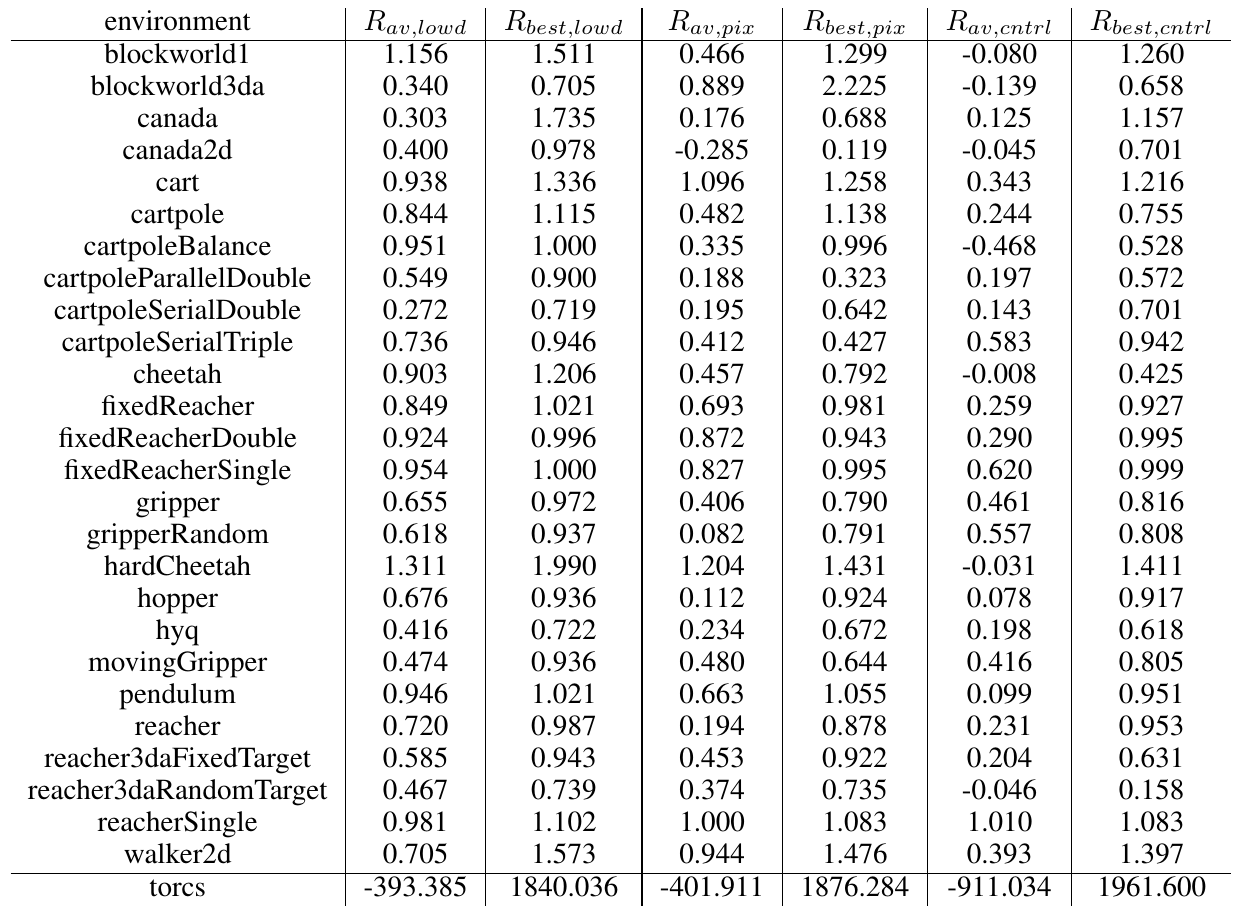
\includegraphics[scale=0.3]{perf_table}
\end{figure}
\end{frame}

\begin{frame}
\frametitle{Results: Estimated Q values}
% \begin{figure}
%     \centering
%     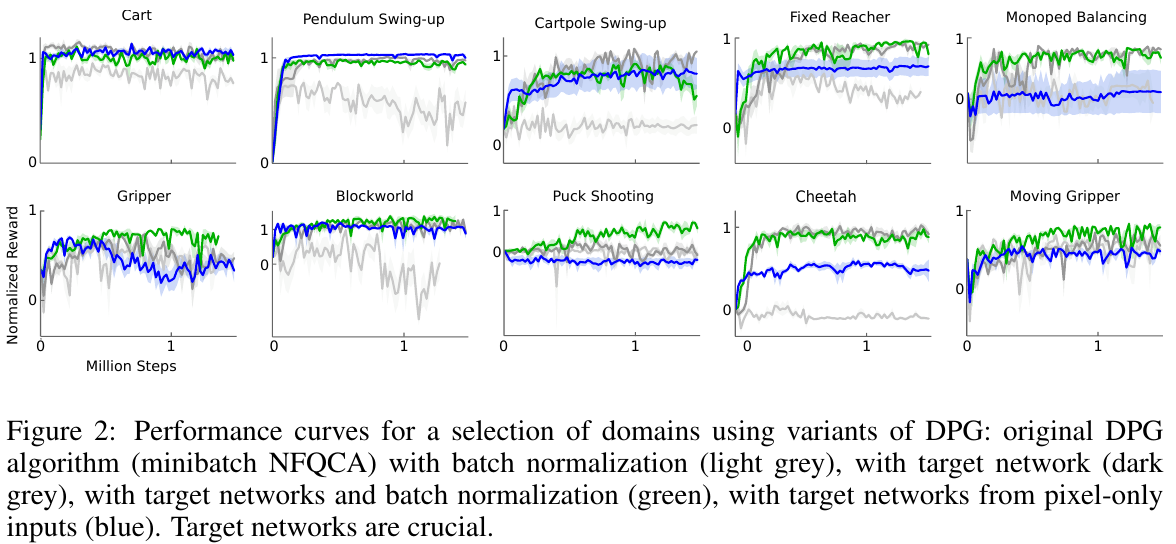
\includegraphics[scale=0.3]{fig_2}
% \end{figure}

\begin{figure}
    \centering
    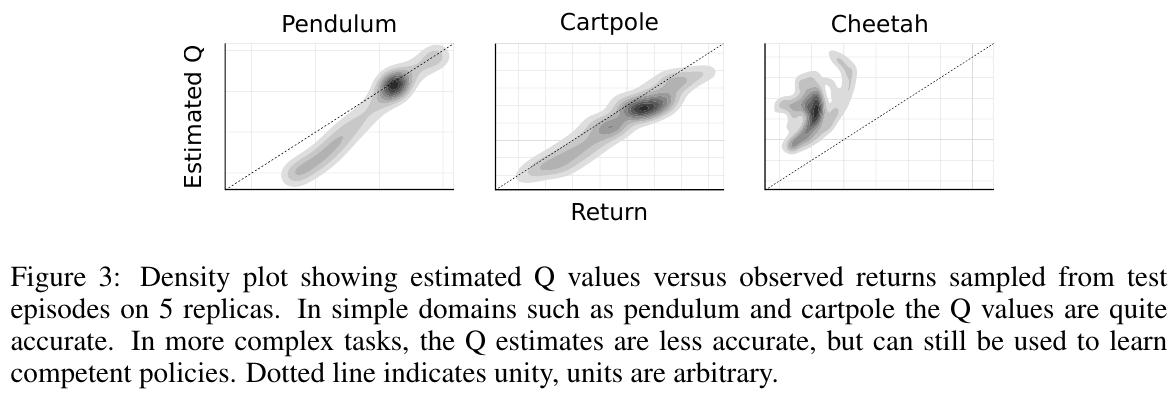
\includegraphics[scale=0.35]{fig_3}
\end{figure}

\end{frame}

\begin{frame}
\frametitle{Results: In words...}

\begin{itemize}
  \item able to find policies whose performance is \textbf{competitive} \\
  with those found by a planning algorithm with full access to the dynamics of the domain and its derivatives.
  \item for many of the tasks the algorithm, can learn policies end-to-end: directly from raw pixel inputs.
  \item in some simpler tasks, learning policies from pixels is just as fast as learning using the low-dimensional state descriptor.\\
  (may also be that the convolutional layers provide an easily separable representation of state space,
  which is straightforward for the higher layers to learn on quickly)
\end{itemize}

See: supplemental video!
\end{frame}
